\documentclass{llncs}

\newif\ifnoTBD \noTBDfalse

% Uncomment to remove TBD macros
%\noTBDtrue

\ifx\pdftexversion\undefined
  \usepackage[dvips]{graphicx}
\else
  \usepackage[pdftex]{graphicx}
  \usepackage{epstopdf}
\fi

\ifnoTBD
\def\TBD#1{\typeout{TBD not done: #1}}
\else
\def\TBD#1{\textcolor{blue}{TBD: #1}}
\AtEndDocument{\typeout{ *** ATTENTION: compilation is in DRAFT
    mode. There might still be TBD that appear in the document ***}}
\fi

\usepackage[usenames]{color}
\usepackage{xspace}
\usepackage{listings}
%\usepackage{type1cm}
\usepackage{eso-pic}
\usepackage{subfigure}
%\usepackage{multirow}
\usepackage{url}
\usepackage{latexsym}
%\usepackage{hyperref}
\usepackage{comment}
\usepackage{algorithmic}
\usepackage{algorithm}
\newcommand{\INDSTATE}[1][1]{\STATE\hspace{#1\algorithmicindent}}

%\hypersetup{%
%  pdftitle={},
%  pdfauthor={George Bosilca},
%  pdfkeywords={network scheduling}
%  bookmarksnumbered, pdfstartview={FitH},
%  linkbordercolor={0 0 0},
%  citebordercolor={0 0 0},
%  urlbordercolor={0 0 0},
%  pdfborder={0 0 0},colorlinks={true},
%  linkcolor={0 0 0},
%  urlcolor=none,
%  citecolor=white
%}%

%\setlength{\oddsidemargin}{0in}   % origin is (1",1") from top-left corner
%\setlength{\evensidemargin}{0.0in}
%\setlength{\textwidth}{6.5in}
%\setlength{\textheight}{9in}
%\setlength{\topmargin}{0.0in}
%\setlength{\headheight}{0pt}
%\setlength{\headsep}{0pt}

\newcommand{\ompi}{Open\,MPI\xspace}
\newcommand{\ftla}{FT-LA\xspace}
\newcommand{\scalapack}{ScaLAPACK\xspace}
%\newcommand{\abft}{Algorithmic Based Fault Tolerance\xspace}
\newcommand{\abft}{ABFT\xspace}
\newcommand{\cof}{CoF\xspace}

\usepackage{algorithmic}
\usepackage{algorithm}
\usepackage{color}
%\usepackage{amsthm}
\usepackage{amsfonts} 
\usepackage{amssymb,amsmath} 
\usepackage{graphicx}
\usepackage[strings]{underscore}

\begin{document}

\title{A Checkpoint-on-Failure Protocol for Algorithm-Based Recovery in Standard MPI}
%\title{Enabling Algorithm-Based Recovery in Standard MPI with Checkpoint-on-Fault}
\author{            Wesley Bland \and
                    Peng Du \and
                    Aurelien Bouteiller \and
                    Thomas Herault \and
                    George Bosilca \and
                    Jack J. Dongarra}
\institute{
                    Innovative Computing Laboratory, University of Tennessee\\
					1122 Volunteer Blvd., Knoxville, TN 37996-3450, USA\\
					\email{\{bland, du, bouteill, herault, bosilca, dongarra\}@eecs.utk.edu}}

\maketitle

\begin{abstract}

As recent research has demonstrated, it is becoming a necessity for large scale
applications to have the ability to tolerate process failure during an
execution. As the number of processes increases, checkpoint/restart fault
tolerance approaches requiring large concurrent state checkpointing become untenable and radically new
methods to address fault tolerance are needed. This work addresses these
challenges by proposing a novel approach to a minimalistic fault discovery and
management model.  Such a model allows application to run to
completion despite fail-stop failures. As a proof of concept, in addition to the
proposed fault tolerance model, an implementation in the context of the \ompi
library is provided, evaluated and analyzed.
% as well as providing a corresponding implementation in the context of the
% \ompi project.  allow applications to discover and tolerate failures while
% continuing execution, all while minimizing application involvement. It
% includes modifications to the \ompi runtime as well as MPI library to give the
% user options when deciding how best to implement fault tolerance.

\end{abstract}


%\begin{IEEEkeywords}
%Fault Tolerance, Message Passing Interface, ABFT, On-Demand Checkpointing
%\end{IEEEkeywords}

\section{Motivation} \label{sect:intro}

Fault tolerance is an increasingly necessary consideration in High Performance Computing (HPC). As machine sizes increase past hundreds of thousands of computing cores\footnote{http://www.top500.org} into the millions of computing resources, the likelihood of failures also increases. Observed failures rates are reaching between 1.8 and 3.6 failures per day on a system of only 635 nodes. This research confirms what has become an accepted reality of HPC going forward. Failures will occur at an increasing rate and for large scale applications to be useful, the failures will need to be handled in software while allowing the applications to continue running relatively uninterrupted.

This realization has lead to much research to attempt to solve the problems presented by the necessity for fault tolerance. The first and most well understood form of fault tolerance is rollback-recovery using periodic checkpointing. This form of fault tolerance has been widely adopted and works well for small scale machines where failure rates are expected to be relatively low. However, at larger scales, even with more reliable hardware, the  time spent performing checkpointing operations is expected to exceed the amount of time spent performing useful computation. To resolve this problem, we turn to Application Based Fault Tolerance (ABFT).

ABFT changes the way applications recover from failure. Rather than loading a previous checkpoint from disk and restarting an entire application, the algorithm itself recovers from the loss of a process and continues without the need to perform costly, large-scale checkpointing operations. The exact method used to recover from failures changes from application to application, but all applications have some requirements in common. The programming model and environment, together with the supporting runtime, need to provide basic functionality in order to allow applications to build a comprehensive fault management solution.

This is a challenging requirement. Most applications continue to use message passing to perform communication between processes, and in the message passing paradigm, collective communication is a popular and necessary way for groups of processes to communicate efficiently. However, collective communication also creates problems when trying to maintain the functionality of the communication library following a process failure due to the complex communication patterns and topologies that must be repaired. 

In addition to maintaining a functional communication library with scalable fault tolerance mechanisms, a fault tolerance solution must also provide extensibility. Because ABFT takes different forms for different applications, the fault tolerance provided by the communication library should also be able to adapt. For example, while one type of application may work best with a transactional model of fault tolerance where sections of the application are re-executed when recovery is necessary, a master-slave type of application may choose to simply spawn a replacement for any process which fails and continue on without needing further recovery.

To this end, we have modified a runtime system to support two new forms of fault tolerance within the message passing paradigm which can provide a suite of tools necessary for developers to include resilience in their applications. Due to size restrictions, details on the work implementing a resilient runtime can be found in~\cite{Bland:CCGrid12}.
\section{Background \& Related Work}
\label{sect:background}

% Discuss some MPI-3 related proposals and issues

%Among the issues
%raised during the readings of the proposals, were the fact that these
%approaches will still incur a significant overhead on failure free
%operations, by requiring periodic \emph{consensus}

\subsection*{Background}

Message passing is the dominant form of communication used in parallel
applications, and MPI is the most popular library used to implement
it. However, as fault tolerance becomes a growing concern for
application developers, users have encountered some challenges with
the current MPI Standard that limit their options of fault tolerance
methods. The primary form of fault tolerance today is to periodically
write a checkpoint to disk.  While this method is effective in
allowing applications to recover from failures by restarting the work
from a previously saved point, it causes serious concerns on the
scalability~\cite{ExaScaleResilience09}. Moreover, such proactive
approach to fault tolerance requires a good idea of how many faults
might hurt the system, with which frequency and on what nodes. Many
works have discussed the optimal checkpointing period in the hope that
as few as possible of these preventive actions are taken by the
application~\cite{Young:1974, Gelenbe:1979, Plank01, Daly:2006,
  PreventiveCheckpointing11}. Unlike these works, the work presented
here focuses on {\it forward recovery}: checkpoint actions are taken
only {\emph after} a failure is detected, make it unnecessary to
hypothesize on an optimal checkpoint interval. The checkpoint interval
is optimal, by definition, as there will be one checkpoint interval by
effective fault.

An alternative approach to rollback recovery is to take advantage of
the properties of the application to design it as naturally fault-tolerant. This
technique is traditionally called \abft \cite{huang1984algorithm}. The
algorithm itself includes modifications, or additional steps, to cope
with the loss of some of its data. It includes a modification of the
algorithm, usually to maintain redundant information in the data
during the life of the application, and a recovery procedure that
works only with the data remaining after the failure is detected, and
reconstructs the missing data using additional computation and
communication. To support such an algorithm, the underlying
programming environment must however provide a way to communicate
after the failure occurs on one of the processes.

The current MPI Standard (MPI-2.2,~\cite{MPI22}) does not provide
significant help to deal with that type of behavior. Section~2.8
states in the first paragraph: ``\emph{MPI does not provide mechanisms
  for dealing with failures in the communication system. [...]
  Whenever possible, such failures will be reflected as errors in the
  relevant communication call. Similarly, MPI itself provides no
  mechanisms for handling processor failures.}'' Failures, be they due
to a broken link or a dead process are considered as resource
errors. Later, in the same section: ``\emph{This document does not
  specify the state of a computation after an erroneous MPI call has
  occurred. The desired behavior is that a relevant error code be
  returned, and the effect of the error be localized to the greatest
  possible extent.}'' So, for the current standard, process or
communication failures are to be handled as errors, and the behavior
of the MPI application after an error has been returned is left
unspecified by the standard. However, the standard does not prevent
implementations to go beyond its requirements, and on the contrary,
encourages high-quality implementations \emph{to return} errors once a
failure is detected.

Unfortunately, most of the implementations of the MPI Standard have
taken the path of considering process failures as unrecoverable
errors, and the processes of the application are most often killed by
the runtime system, when a failure hits any of them. The runtime
system then returns with an error code, signaling the failure of the
run, leaving no other choice to the user but to run a new parallel
execution.

The MPI forum is currently examining options for the future direction
of MPI for MPI-3. One of the workgroups is dedicated to propose a
standard form of MPI-supported fault tolerance. The proposal outlines
a method of run-through stabilization which allows the application to
acknowledge and repair communications, both collectively and between
specific ranks in a point-to-point way~\cite{Hursey11MPI3FT}. The
emphasis of the proposal is a set of "validation" functions which the
application is required to call to repair and re-enable communication within
an MPI communicator containing a failed process. To repair point to
point wildcard receives, the application needs to collectively call the function
MPI\_COMM\_REENABLE\_ANY\_SOURCE. To repair collective communication
within a communicator, the application needs to call the function
MPI\_COMM\_VALIDATE.  These functions give the MPI implementation an
opportunity to acknowledge failures and discover or ensure that other
MPI processes also acknowledge the same failures. It also gives the
MPI library a chance to repair communication channels between
remaining processes, optimizing communication topologies if possible
and necessary.

While this method of fault tolerance is sufficient for \abft, it is
not without its drawbacks. The calls necessary to recover from
collectives incur a non-trivial overhead even during the fault free
case. MPI\_COMM\_VALIDATE requires a distributed consensus algorithm
which is currently best implemented at log
scale~\cite{Hursey11LogConsensus}. While this level of overhead is
better than the current state of the art of periodic checkpointing, it
still presents a significant cost that not all applications want or
need to pay to check the validity of the communicators. Most
importantly, this proposal does not yet include process recovery,
which is left to a future proposal to the MPI forum.

% Discuss issues in general with FT-MPI like approaches, besides the 
% sheer problem of standard adoption

% Explain why it is not believed that ABFT can perform without REPLACE 
% or BLANK, or leave it for next section ?

\subsection*{Related Work}

FT-MPI~\cite{fagg2000ft} is an MPI-1 implementation which added
extensions to the MPI standard to give users options for their
\abft. FT-MPI proposed to change the MPI semantics of some of the
calls, to enable continuing the execution of the parallel application
after a failure hits the system, and to rebuild the communicators, thus
re-enabling communications. This approach has been proven successful,
and some applications have been implemented relying on the features of
FT-MPI. However, these modifications of the standard were not imported
in the official MPI standard, and no other MPI implementation took the
same approach. The lack of large distribution of the FT-MPI
implementation prevented a large base of users from implementing their
solution based on this proposition.

%  One of
% the solutions implemented in FT-MPI was to introduce a new MPI\_Errhandler
% called MPI\_ERRORS\_BLANK. This MPI\_Errhandler replaced the position of the
% failed processes inside a communicator with MPI\_PROC\_NULL. By using this
% semantic, the remaining MPI calls could function normally as communication with
% MPI\_PROC\_NULL always succeeds. When FT-MPI encountered a fault, it destroyed
% all MPI Communicators and required that the application recreate them to account
% for the failed processes. While this was a useful step in allowing the most
% level of flexibility from the application's perspective, it made recovery very
% complex and added a large overhead.

% FT-MPI is another form of fault tolerance that can be successful for some, but in
% applications that require that all processes be running to reach successful
% completion, having a hole in the communicator is not a valid solution. The
% failed processes need to somehow be recovered.

%\TBD{Anything needed from the QR side of things?}

Besides the works that have been cited previously to present the
problem statement, the different approaches that have been proposed,
and how this approach is original, the article by W. Gropp and E. Lusk
in 2004 \cite{Gropp:2004:FTM:1080704.1080714} is the work closest to
the On-Demand Checkpointing, from the MPI requirement perspective.  In
this article, the authors explain how the standard can be interpreted,
or slightly modified, to allow for a form of fault tolerance. They
consider different approaches: periodical checkpointing; using
inter-communicators and separate MPI applications to contain an error
in an MPI application; modifying the MPI semantics; or propose new
extensions. However, the last three propositions demand more from the
MPI implementation than we require in this work: for example, the MPI
library is supposed to continue its normal execution, if the error was
located in another MPI application, connected with the one subject to
the error through an inter-communicator. In our work we do not even
require such a step: the only
demand on the MPI implementation is that it does not forcibly kill the
living processes without letting them take a checkpoint, but returns
an error. Once this is ensured, no requirement from any MPI call is
needed.

Moreover, we illustrate the well soundness of our approach using a
non-trivial algorithm: a QR factorization, that is made fault tolerant
using the modified \ompi, and the On-Demand Checkpointing
technique. We demonstrate that this approach is functional, and
evaluate its performance at large scale.

\section{Enabling Algorithm-Based Fault Tolerance in MPI}
\label{sect:ompi}

\subsection{The Checkpoint-on-Failure Protocol}

In this paper, we advocate that an extremely efficient form of fault tolerance
can be implemented, strictly based on the MPI standard, for applications capable
of taking advantage of forward recovery. \abft methods are an example of forward
recovery algorithms, capable of restoring missing data from redundant information
located on other processes.  This forward recovery step requires communication
between processes, and we acknowledge that, in light of the current standard,
requiring the MPI implementation to maintain service after failures is too
demanding. However, a high-quality MPI library should at least allow the application to regain control following a process failure. We note
that this control gives the application the opportunity to save its state and
exit gracefully, rather than the usual behavior of being aborted by the MPI
implementation.

\begin{algorithm}
\caption{The Checkpoint-on-Failure Protocol}
\label{alg:on-demand-alg}\label{fig:idea}
\centering
\begin{minipage}[b]{.55\linewidth}
	\begin{enumerate}\sffamily\small
		\item MPI returns an error on surviving processes 
		\item Surviving processes checkpoint
		\item Surviving processes exit
		\item A new MPI application is started
		\item Processes load from checkpoint (if any)
		\item Processes enter \abft dataset recovery
		\item Application resumes
	\end{enumerate}
\end{minipage}
\hfill
\begin{minipage}[b]{.39\linewidth}
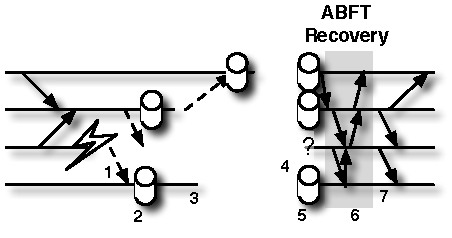
\includegraphics[width=\linewidth]{figures/idea.pdf}
%\caption{Failure recovery execution diagram of On-Demand Checkpointing\label{fig:idea}}
\end{minipage}
\end{algorithm}

Based on these observations, we propose a new approach for supporting
\abft applications, called Checkpoint-on-Failure (\cof).
Algorithm~\ref{alg:on-demand-alg} presents the steps involved in the
\cof method. In the associated explanatory figure, horizontal lines
represent the execution of processes in two successive MPI applications.
When a failure eliminates a process, other processes are notified and
regain control from ongoing MPI calls (1). Surviving processes assume
the MPI library is dysfunctional and do not further call MPI operations
(in particular, they do not yet undergo \abft recovery). Instead, they
checkpoint their current state independently and abort (2, 3). When
all processes exited, the job is usually terminated, but the user (or a
managing script, batch scheduler, runtime support system, etc.) can
launch a new MPI application (4), which reloads processes from
checkpoint (5). In the new application, the MPI library is functional
and communications possible; the \abft recovery procedure is called to
restore the data of the process(es) that could not be restarted from
checkpoint (6). When the global state has been repaired by the \abft
procedure, the application is ready to resume normal execution.

%AURELIEN: true enough, but I need to  cut lines. 
%If another failure hits the system during the recovery, the local states
%are not updated, and the relaunch starts from the beginning. If another
%failure hits the system after the \abft recovery, the same procedure is
%followed to handle it.

Compared to periodic checkpointing, in \cof, a process
pays the cost of creating a checkpoint only when a failure, or multiple simultaneous 
failures have happened,
hence an optimal number of checkpoints during the run (and no checkpoint
overhead on failure-free executions). Moreover, in periodic checkpointing,
a process is protected only when its checkpoint is stored on safe,
remote storage, while in \cof, local checkpoints are
sufficient: the forward recovery algorithm reconstructs datasets of
processes which cannot restart from checkpoint. 
Of course, \cof also exhibits the same overhead as the standard \abft approach: the
application might need to do extra computation, even in the absence of
failures, to maintain internal redundancy (whose degree varies with the 
maximum number of simultaneous failures) used to recover data damaged
by failures. However, \abft techniques often demonstrate excellent
scalability; for example, the overhead on failure-free execution of the
\abft QR operation (used as an example in Section~\ref{sec:ftla}) is inversely
proportional to the number of processes.

\subsection{MPI Requirements for Checkpoint-on-Failure}\label{sec:interface}

\paragraph*{Returning Control over Failures:} In most MPI
implementations, MPI\_ERRORS\_ABORT is the default (and often, only
functional) error handler. However, the MPI standard also defines the
MPI\_ERRORS\_RETURN handler. To support \cof, the MPI
library should never deadlock because of failures, but invoke the error handler, at least on
processes doing direct communications with the failed process. The
handler takes care of cleaning up at the library level and returns
control to the application.

\paragraph*{Termination After Checkpoint:} A process that detects a
failure ceases to use MPI. It only checkpoints on some storage and
exits without calling MPI\_Finalize. Exiting without calling
MPI\_Finalize is an error from the MPI perspective, hence the failure
cascades and MPI eventually returns with a failure notification on every process, which triggers their own checkpoint procedure and termination.

\subsection{\ompi Implementation\label{sec:mpi}}

\ompi is an MPI 2.2 implementation architected such that it contains two
main levels, the runtime (ORTE) and the MPI library (OMPI). As with most
MPI library implementations, the default behavior of \ompi is to abort
after a process failure. This policy was implemented in the runtime
system, preventing any kind of decision from the MPI layer or the
user-level. The major change requested by the \cof protocol was to make the
runtime system resilient, and leave the decision in case of failure to
the MPI library policy, and ultimately to the user application.

\paragraph*{Failure Resilient Runtime:} The ORTE runtime layer provides
an out-of-band communication mechanism (OOB) that relays messages based
on a routing policy. Node failures not only impact the MPI
communications, but also disrupt routing at the OOB level. The
default routing policy in the Open MPI runtime has been amended to allow
for self-healing behaviors; this effort is not entirely 
necessary, but it avoids the significant downtime imposed by a complete 
redeployment of the parallel job with resubmission in queues. The 
underlying OOB topology is automatically updated to route around failed processes. In some routing topologies,
such as a star, this is a trivial operation and only requires excluding
the failed process from the routing tables. For more elaborate
topologies, such as a binomial tree, the healing operation involves
computing the closest neighbors in the direction of the failed process
and reconnecting the topology through them. The repaired topology is
not rebalanced, resulting in degraded performance but complete
functionality after failures. Although in-flight messages that were
currently ``hopping'' through the failed processes are lost, other
in-flight messages are safely routed on the repaired topology. Thanks to self-healing topologies, the runtime remains responsive, even when MPI processes leave. 
%This persistent
%runtime avoids losing the batch scheduler reservation and eliminates the cost
%of redeploying the runtime infrastructure.
% It also remains available for spawning replacement MPI processes, and to
% access locally stored checkpoints.

\paragraph*{Failure Notification:} The runtime has been augmented with a
failure detection service. To track the status of the failures, an
incarnation number has been included in the process names. Following a
failure, the name of the failed process (including the incarnation
number) is broadcasted over the OOB topology. By including this
incarnation number, we can identify transient process failures, prevent
duplicate detections, and track message status. ORTE processes monitor
the health of their neighbors in the OOB routing topology. Detection of
other processes rely on a failure resilient broadcast that overlays on
the OOB topology. This algorithm has a low probability of creating a
bi-partition of the routing topology, hence ensuring a high accuracy of
the failure detector. However, the underlying OOB routing algorithm has
a significant influence on failure detection and propagation time, as
the experiments will show. On each node, the ORTE runtime layer forwards
failure notifications to the MPI layer, which has been modified to
invoke the appropriate MPI error handler.
%(MPI\_ERR\_RETURNS, or a custom error handler). MPI calls are interrupted and
%the application regains control. The MPI library purges internal queues and
%state, to minimize the size of checkpoint.

\section{Example: the QR Factorization}
\label{sec:ftla}

In this section, we propose to illustrate the applicability of \cof by
considering a representative routine of a widely used
class of algorithms: dense linear factorizations. The QR factorization
is a cornerstone building block in many applications, including solving
$Ax=b$ when matrices are ill-conditioned, computing eigenvalues, least
square problems, or solving sparse systems through the GMRES iterative
method. For an $M\times N$ matrix $A$, the QR factorization produces $Q$ and
$R$, such that $A=QR$ and $Q$ is an $M\times M$ orthogonal matrix and
$R$ is an $M\times N$ upper triangular matrix. The most commonly used
implementation of the QR algorithm on a distributed memory machine comes
from the ScaLAPACK linear algebra library~\cite{dongarra1997scalapack},
based on the block QR algorithm. It uses a 2D block-cyclic distribution
for load balance, and is rich in level 3 BLAS operations, thereby
achieving high performance.

%$Q$ is stored
%under the lower diagonal of the input matrix in the form of a $WY$
%representation of the Householder transformation
%products~\cite{schreiber1989storage,bischof1985wy}.

\subsection{\abft QR Factorization}

In the context of FT-MPI, the ScaLAPACK QR algorithm has been rendered fault
tolerant through an \abft method in previous works~\cite{pengduppopp12}. This
\abft algorithm protects both the left ($Q$) and right ($R$) factors from fail-stop
failures at any time during the execution.  At the time of failure, every surviving process is notified by FT-MPI. FT-MPI
then spawns a replacement process that takes the same grid coordinates in the
$P\times Q$ block-cyclic distribution. Missing checksums are recovered from
duplicates, a reduction collective communication recovers missing data blocks in
the right factor from checksums. The left factor is protected by the Q-parallel
panel checksum, it is either directly recovered from checksum, or by
recomputing the panels in the current Q-wide section
(see~\cite{pengduppopp12}). Although this algorithm is fault tolerant, it
requires continued service from the MPI library after failures -- which is a
stringent requirement that can be waived with \cof.

\subsection{Checkpoint-on-Failure QR}

\paragraph*{Checkpoint Procedure:} Compared to a regular \abft
algorithm, \cof requires a different checkpoint
procedure. System-level checkpointing is not applicable, as it would result
in restoring the state of the broken MPI library upon restart. Instead,
a custom MPI error handler invokes an algorithm specific checkpoint
procedure, which simply dumps the matrices and the value of important
loop indices into a file.

\paragraph*{State Restoration:} A ScaLAPACK program has a deep call
stack, layering functions from multiple software packages, such as
PBLAS, BLACS, LAPACK and BLAS. In the FT-MPI version of the algorithm,
regardless of when the failure is detected, the current iteration of the
algorithm must be completed before entering the recovery procedure. This
ensures an identical call stack on every process and a complete update
of the checksums. In the case of the \cof protocol, failures interrupt
the algorithm immediately, the current iteration cannot be completed due
to lack of communication capabilities. This results in potentially
diverging call stacks and incomplete updates of checksums. However,
because failure notification happens only in MPI, lower level, local
procedures (BLAS, LAPACK) are never interrupted.

To resolve the call stack issue, every process restarted from checkpoint
undergoes a ``dry run'' phase. This operation mimics the loop nests of the
QR algorithm down to the PBLAS level, without actually applying
modifications to or exchanging data. When the same loop indices as
before the failure are reached, the matrix content is loaded from the
checkpoint; the state is then similar to that of the FT-MPI based \abft
QR after a failure. The regular recovery procedure can be applied: the
current iteration of the factorization is completed to update all
checksums and the dataset is rebuilt using the \abft reduction.

\begin{comment}
	
A special situation where failure occurs during 
lower level routines such as PDLARFB is also addressed. This critical 
situation has not been  
covered by any previous work for the complexity it introduces.
	
\subsection{Failure in PBLAS routines}
An important condition for the effectiveness of \abft is the
completion of the current iteration. When a failure interrupts the
program execution during an iteration, the checksum ends up in
intermediate form and as a result cannot be used for recovery.  This
problem worsens when a failure occurs during a lower level routine, 
like a PBLAS, causing a partial trailing matrix update. In this case, updates have been applied to parts of the dataset, possibly without having updated accordingly the corresponding checksums. In the case of the QR algorithm, this problem
is solved by saving the local state when a failure is detected in
PDLARFB rather than in PDGEQRF. The recovery
process in this case is described as follow.

\begin{figure}[b]
	\centering
	\subfigure[After the first step: $A_{2}^{T}V$]{\label{fig:gull1}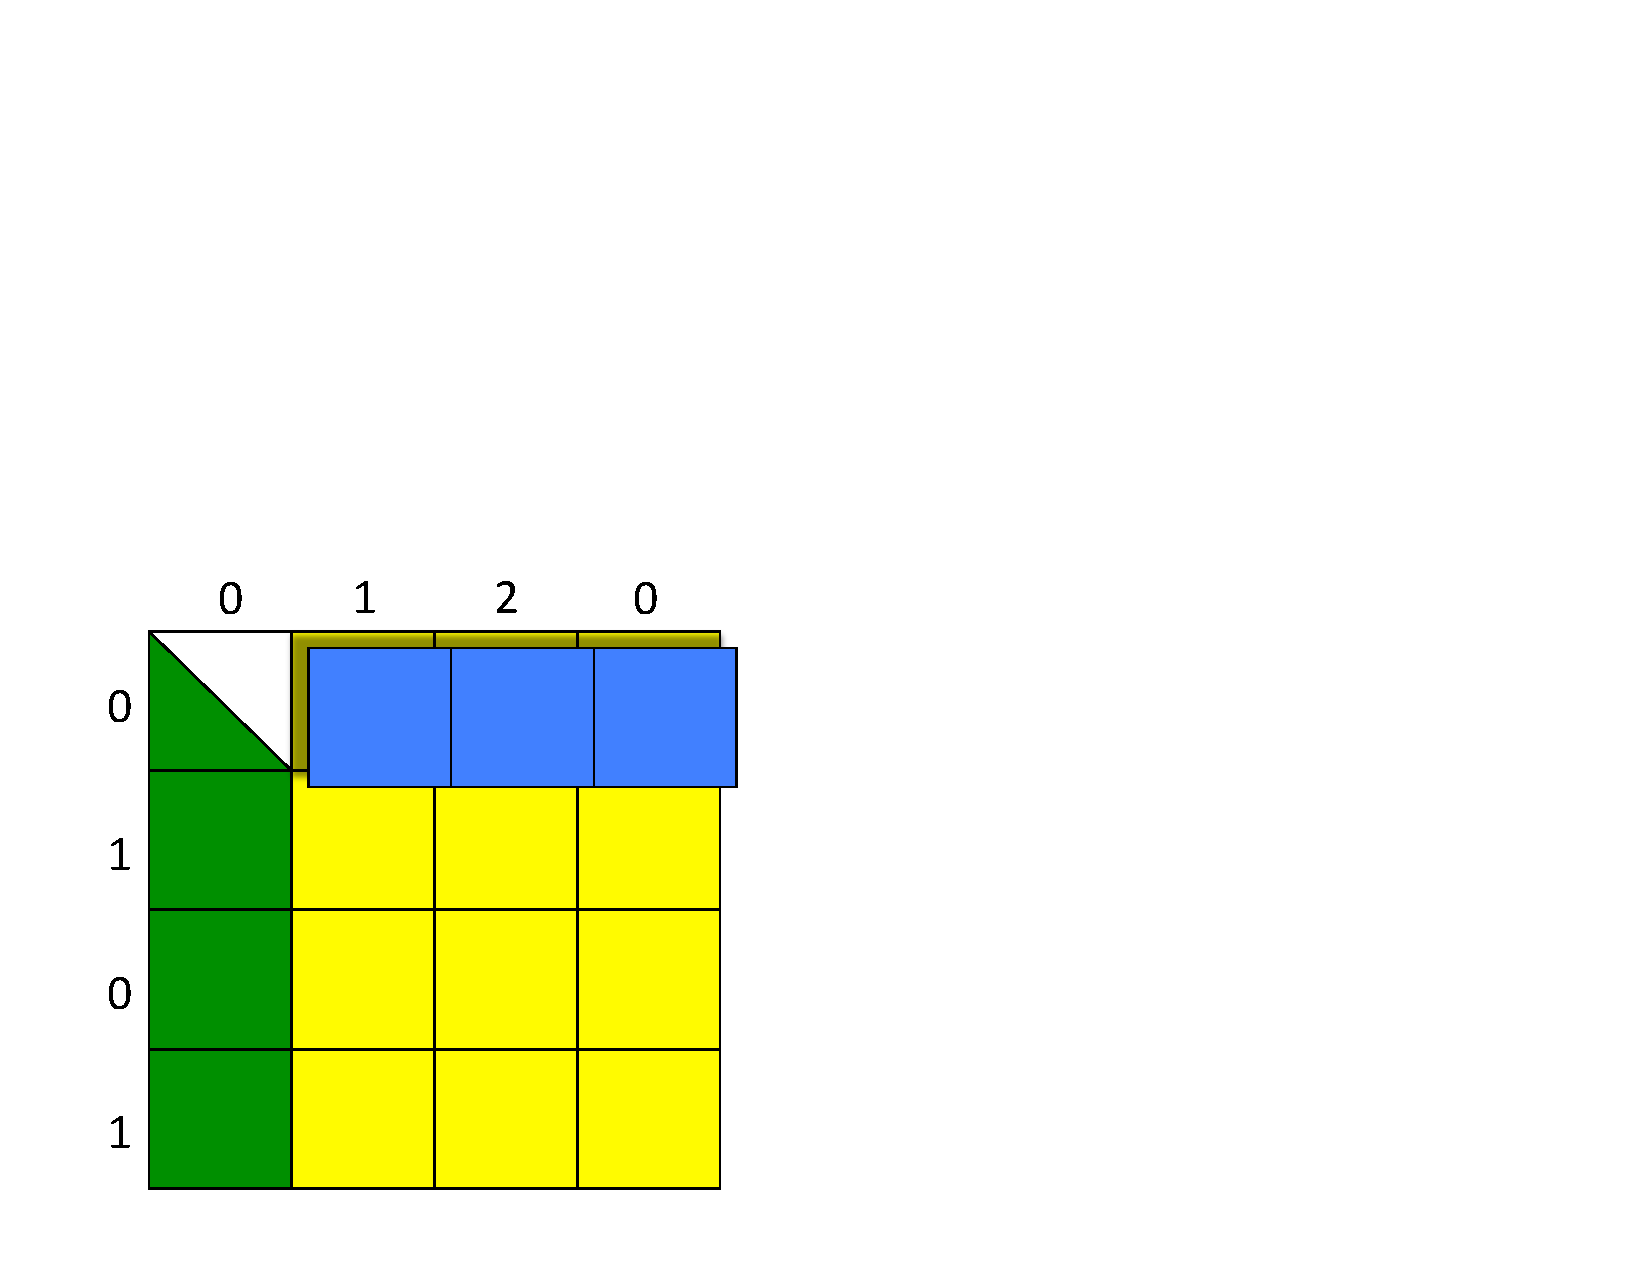
\includegraphics[totalheight=0.15\textheight, width=0.18\textwidth,viewport=10 10 360 360, clip]{figures/pdlarfb_step1}
	\label{fig:pdlarfb_step1}}
	%\line(0,1){100}
	\subfigure[$A_{2}-V\tilde{W}^{T}$]{\label{fig:gull2}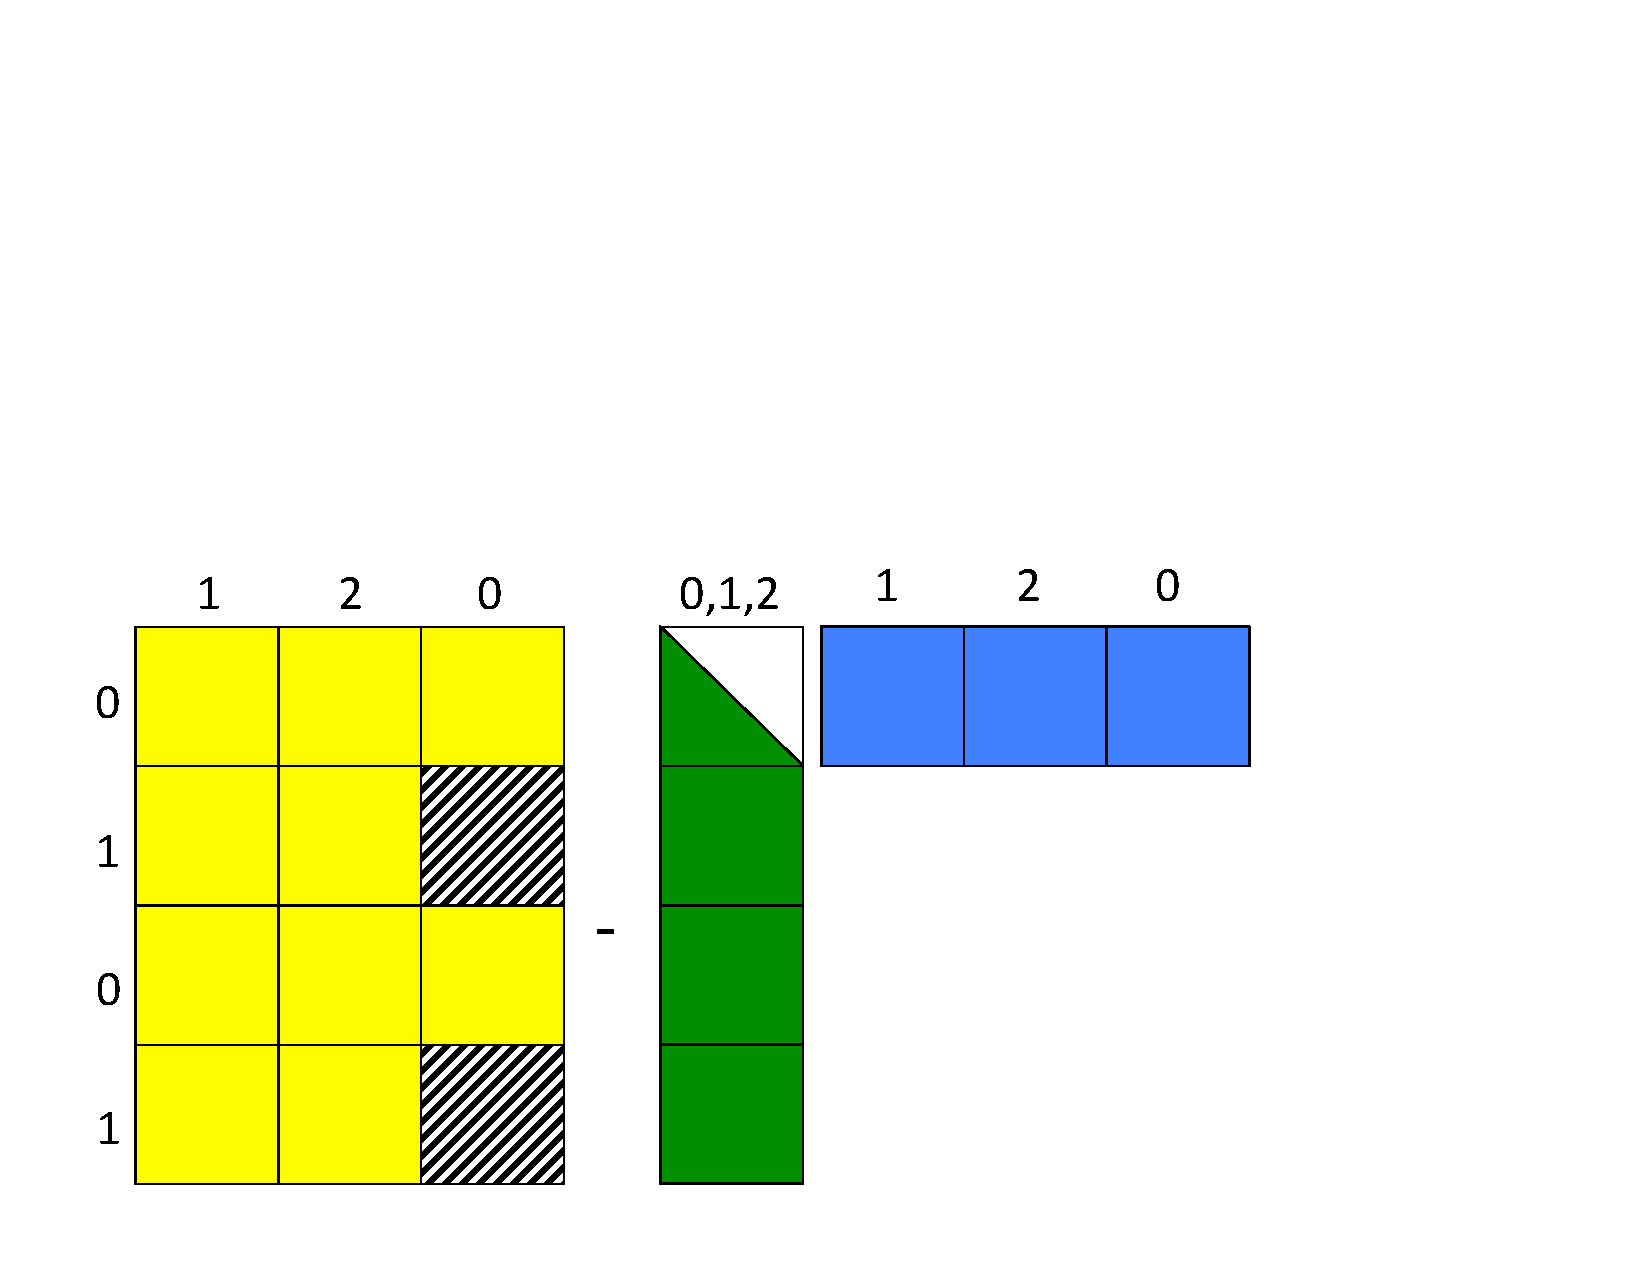
\includegraphics[totalheight=0.15\textheight, width=0.3\textwidth,viewport=10 10 600 360, clip]{figures/pdlarfb_step2}
	\label{fig:pdlarfb_step2}}
	\caption{PDLARFB}
\end{figure}

As shown in Equation (\ref{eqn:qr-trailing}), the trailing update of QR carries
out operation $Q^{T}A_{2}=(I-VT^{T}V^{T})A_{2}\rightarrow
\tilde{A}_{2}$. The right arrow means the updated trailing matrix is
written in-place to $A_{2}$. The trailing matrix update of QR is
similar to PDGEMM for LU which has been shown to hold the checksum
relationship only at the end~\cite{pengduppopp12}. Therefore the procedure
to recover from a failure in PDLARFB is:
\begin{enumerate}
\item Survived processes mark the progress and dump critical data to disk 
\item After re-spawning, all processes dry-run to the failure point
\item All except the replacement process load checkpoint from disk 
\item All processes resume computing from the failure point to the end of PDLARFB
\item At the exit of PDLARFB, recover all lost data in checksum and the whole matrix
\item Execution of PDGEQRF returns to normal
\end{enumerate}
The 'dry-run' step is to re-establish the calling stack of all processes to
the failing point. Therefore PBLAS and ScaLAPACK routines for
computing, for example, PDGEQR2, PDLARFT, etc. are skipped over during 
the dry run.

The recovery is demonstrated with an example of a $4\times 4$ blocks
matrix on a $2\times 3$ grid where failure occurs during PDLARFB.

PDLARFB implements $Q^{T}A_{2}=(I-VT^{T}V^{T})A_{2}$ in three steps:
\begin{enumerate}
\item $W\leftarrow V^{T}A_{2}$
\item $\tilde{W}\leftarrow W\times T$
\item $\tilde{A}_{2}\leftarrow A_{2}-V\tilde{W}^{T}$
\end{enumerate}
Suppose the failure occurs right after step 1 on process (1,0). 
In step 1, as shown in figure~\ref{fig:pdlarfb_step1}, $V$ is stored
in the green trapezoid and $A_{2}$ is in the yellow blocks. $V$ is
first broadcast row-wise to all columns, then GEMM is called on each
process that owns $A_{2}$ with the local $V$ and $A_{2}$. Finally, the
result is produced with column-wise block summation and the result is
stored on the first row of processes that process the first row of
$A_{2}$ (blue blocks).  From the MPI facilities presented in
Section~\ref{sec:mpi}, the failure location is broadcasted to all 
surviving processes and matrix data are dumped to the disk, including
peripheral data like the TAU array and workspace. Surviving processes
also keep a record on whether they have finished the DGEMM in step 1.

After critical data is saved to disk, the program exits and is
re-spawn with a replacement process in the failed process's
location. The re-launched program dry-runs to the failure point in
step 1 of PDLARFB. All previously surviving processes load their
checkpoint from disk while the replacement process stays with its
blank data. Then the program resumes execution of PDLARFB. Since
failure is on process (1,0), $W$ survives the data loss.

Step 2 of PDLARFB is $W\times T$ where $W$ is the blue blocks in
figure~\ref{fig:pdlarfb_step1} and $T$ is a $nb\times nb$ upper
triangular matrix.  Since $T$ resides on each process in the row that
owns $W$, the correctness of $T$ can be always guaranteed, and
therefore $\tilde{W}$ has no lost block in it after calling
DTRMM. $\tilde{W}$ is broadcasted column-wise for step 3.

Step 3 of PDLARFB is shown in figure~\ref{fig:pdlarfb_step2}. In
$\tilde{A}_{2}\leftarrow A_{2}-V\tilde{W}^{T}$, besides
$\tilde{W}^{T}$, $V$ is also correct since $V$ has been broadcast
row-wise to all process in step 1, therefore even if blocks of $V$ are
destroyed by the failure, the result on the replacement process can be
recovered from its neighbor processes in the same row. The result of
step 3, also that of PDLARFB, is affected by the incorrect result in
$A_{2}$, expressed in shadowed blocks in
figure~\ref{fig:pdlarfb_step2}. These incorrect blocks remain in the
result of DGEMM in this step. They are fixed later in the recovery process
in PDGEQRF using both the ABFT and Q-parallel checksum.

For PDLARFB, both $V$ and $T$ can be guaranteed correct no matter when
and where failure occurs, the only variable factor is $W$. However if
the failure does punch holes in $W$, more shadow blocks appear in
the result of PDLARFB, and they can still be fixed by the recovery in
PDGEQRF.
\end{comment}

\begin{comment}
\section{Models of Fault Tolerance Approaches\label{sec:model}}

In this section, we present a simple model that we use to evaluate the
efficiency of our approach, when compared to the classical approach of
a coordinated, blocking checkpointing algorithm. For the following,
we will consider an application with a fixed number of processes, and
a fixed amount of work to execute. We consider that without any
fault-tolerance approach enabled, the execution time of this work with
this number of processes is $T$.

The ABFT technique, as proposed in this article, can be characterized
with a few parameters:
\begin{itemize}
\item $C$, the time it takes the living processes, to save their state
  after the failure occurs, exit, and for the runtime system to
  discover that all processes have exited with an error code
\item $\alpha$, a multiplicative factor, that encompasses all costs
  related to making the operation ABFT-capable. Such modification of
  the operation introduces additional operations and communications,
  distributed among the processes. Based on our experience with ABFT,
  we consider, in this model, that these operations introduce a
  slowdown of the execution time that can be captured with a single
  multiplicative factor, $\alpha > 1$.
\item $R$, the time it takes for processes to restart from scratch,
  load the checkpoints of the living processes, exchange the missing
  information, and recover the missing data.
\end{itemize}
Since the number of processors and the problem size are fixed, $C, R,$
and $\alpha$, can all be considered as constants.

Our approach is deterministic, given these assumptions: the time it
takes to complete the execution of the work with a number $n$ of
failures is 
\begin{eqnarray}
T^{ABFT}(n) &=& \alpha T + n ( C + R )
\end{eqnarray}

Indeed, the execution is slowed down by the $\alpha$ parameter to
maintain the different checksums incurred by the ABFT approach, and
each failure triggers first a checkpoint phase, that is immediately
followed by a recovery phase. At the end of the recovery phase, the
algorithm is ready to proceed at the step that follows the failure, so
no additional cost is incurred.

The periodical coordinated blocking checkpointing technique can be
characterized with the following parameters:
\begin{itemize}
\item $c$, the time it takes for all processes to save their state
  when the timer expires
\item $r$, the time it takes all processes to restart from this
  checkpoint (load the checkpoint from file)
\item $t$ is the time interval between two checkpoints. This value is
  usually set to something as close as possible to the expected MTBF,
  to avoid unnecessary overheads. It must be set low enough, though,
  to allow for progress.
\end{itemize}
In the coordinated checkpointing approach, the duration of the
execution depends upon the moment of the failures: if a failure hits
the system just after a checkpoint, no time is lost to recompute the
state between the last checkpoint and the current step of the
computation. If a failure hits the system just before a checkpoint,
then the recovery restarts from the last checkpoint and the last
time interval must be entirely re-executed. To model this, we define
two extreme cases: the best case, noted $T^{CC}_B(n)$ (for Time,
Coordinated Checkpointing, Best case), and $T^{CC}_W(n)$ (for Time,
Coordinated Checkpointing, Worst case). These functions can be defined
recursively as follows:
$$
\left\{\begin{array}{l}
T^{CC}_B(0) = T + c T/t\\
T^{CC}_B(n) = T^{CC}_B(n-1) + r + c r/t\\
\end{array}\right.$$
$$\left\{\begin{array}{l}
T^{CC}_W(0) = T + c T/t\\
T^{CC}_W(n) = T^{CC}_W(n-1) + r + t+ c (r+t)/t\\
\end{array}\right.
$$

The cost on the execution without recovery is to stop the execution
every $t$ times units, and take a checkpoint. The recovery cost
depends upon the case that is considered. In the best case, all
failures will happen just after the last valid checkpoint. Hence the
cost of recovery will be simply the time to load this checkpoint. In
the worst case, all failures will happen just before the next
checkpoint is completed, hence the cost of recovery will be the time
to load the checkpoint, plus the time to redo the missing part of the
execution, every time. Since recoveries increase the duration of the
execution, they also increase the number of checkpoints that are
taken.

We can solve these recursive definitions to obtain the following
general forms:
\begin{eqnarray}
T^{CC}_B(n) &= & (c+t)(n r +T)/t\\
T^{CC}_W(n) & = & (c+t) (n (r+t) + T) /t
\end{eqnarray}

To compare the two models, we can assume that if a local storage is
present, $C \ll c$: in the case of the ABFT approach, if the same
nodes remain accessible to the application to restart its runs, and a
local storage is accessible, saving the checkpoint will be a local,
embarrassingly parallel, operation. The Coordinated Checkpointing
approach, however, cannot rely on local storage: a checkpoint image of
all the nodes, including the failed nodes, will be necessary at
recovery time. Thus, in the best case, a buddy algorithm must be used
if local storage is to be used. Introducing additional communications,
the checkpointing time is expected to be larger in that case.

On the other hand, if a local storage is not accessible, one can
safely assume that $C \sim c$, since they save the same amount of
information (we are considering a user-level checkpointing in both
cases). This checkpointing time can be influenced, in the case of a
shared filesystem, by the number of nodes that checkpoint image
together, but since we assume one failure simultaneously, the fact
that the ABFT algorithm saves one less image might be not significant
at large scale.

Similarly, if no local storage is available, $R \gg r$: they both
incur the communication cost linked to loading the checkpoint image,
but then the ABFT technique needs to introduce additional
communications to recover the state. If a local storage is available,
this will strongly depend on the amount of data saved, and the amount
of communication required by the ABFT algorithm to implement its
recovery. 

Both models present a linear progression with the number of
faults. When $n=0$, the On-Demand Checkpointing approach is slowdown
by the factor $\alpha$, while the periodical Checkpointing approach
incurs a slowdown proportional to $(c+t)/t = 1+c/t$. As was
demonstrated in~\cite{lawn253}, $alpha$ decreases when the number of
processes increase. In the case of the QR factorization, it increases
with the square root of the problem size, to maintain the checksum
operation. $c/t$ is proportional to the duration of the checkpoint
operation, hence to the problem size, and in non-scalable storage
system with the number of processes. Moreover, it is highly dependent
on the $t$ parameter, that is often be set conservatively to guarantee
progress in case of failures.

When the system is subject to failures, the cost of the recovery of
the On-Demand Checkpointing technique is proportional to the number of
failures, and to the duration of the recovery, $R$. As stated above,
this overhead depends on the disk capabilities, but also on the
efficiency of the recovery procedure given by the \abft algorithm, and
on the runtime system of the MPI to detect the incomplete termination,
and launch a new application, efficiently. In the case of $QR$, this
recovery increases with the size of the problem and the square root of
the number of computing elements. The periodical checkpointing
approach on the other hand incurs a recovery cost that is constant,
but must redo part of the execution. A large $t$ parameter in this
case is damageable because it increase the probability that a long
part of the computing time is lost. The On-Demand Checkpointing
technique does not suffer from this parameter, and the cost of
recovery is entirely defined by the size of the problem and the number
of processors.
\end{comment}

\section{Performance Discussion}\label{sec:experiments}

In this section, we use our \ompi and \abft QR implementations to
evaluate the performance of the \cof protocol. We
use two test platforms. The first machine, ``Dancer,'' is a 16-node
cluster. All nodes are equipped with two 2.27GHz quad-core Intel E5520
CPUs, with a 20GB/s Infiniband interconnect. Solid State Drive disks are
used as the checkpoint storage media. The second system is the Kraken
supercomputer. Kraken is a Cray XT5 machine, with 9,408 compute nodes.
Each node has two Istanbul 2.6 GHz six-core AMD Opteron processors, 16
GB of memory, and are connected through the SeaStar2+ interconnect. The
scalable cluster file system ``Lustre'' is used to store checkpoints.

\subsection{MPI Library Overhead}

One of the concerns with fault tolerance is the amount of overhead
introduced by the fault tolerance management additions. Our
implementation of fault detection and notification is mostly implemented
in the non-critical ORTE runtime. Typical HPC systems
feature a separated service network (usually Ethernet based) and a
performance interconnect, hence health monitoring traffic, which happens
on the OOB service network, is physically separated from the MPI
communications, leaving no opportunity for network jitter. Changes to
MPI functions are minimal: the same condition that used to trigger
unconditional abort has been repurposed to trigger error handlers. As
expected, no impact on MPI bandwidth or latency was measured
(Infiniband and Portals results not shown for lack of space). The memory
usage of the MPI library is slightly increased, as the incarnation
number doubles the size of process names; however, this is negligible in
typical deployments.

\subsection{Failure Detection}

According to the requirement specified in Section~\ref{sec:interface}, only
in-band failure detection is required to enable \cof. Processes detecting a
failure checkpoint then exit, cascading the failure to processes communicating
with them. However, no recovery action (in particular checkpointing) can take 
place before a failure has been
notified. Thanks to asynchronous failure propagation in the
runtime, responsiveness can be greatly improved, with a high probability for the
next MPI call to detect the failures, regardless of communication pattern or
checkpoint duration.

\begin{figure}[htb]
\centering 
  \subfigure[Linear OOB Routing]{
    \label{fig:linear}
    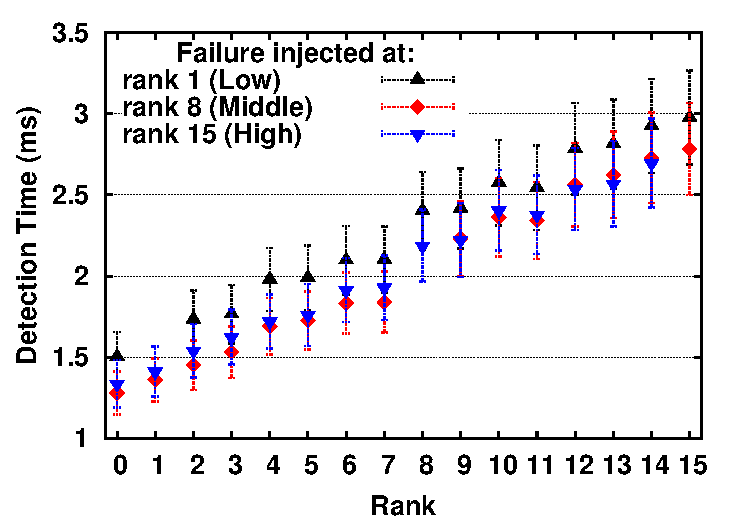
\includegraphics[width=.43\linewidth]{figures/failure_detection_linear_errbars}}
  \hfill
  \subfigure[Binomial OOB Routing]{
    \label{fig:binomial}
    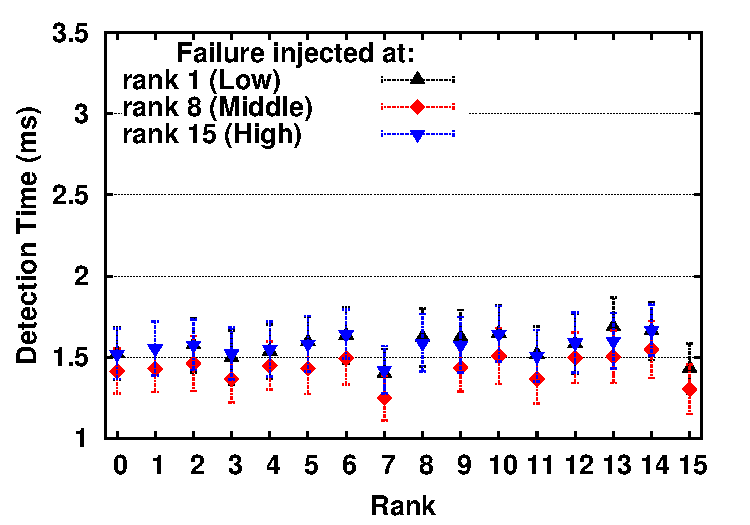
\includegraphics[width=.43\linewidth]{figures/failure_detection_binomial_errbars}}\vspace{-.2cm}
\caption{Failure detection time, sorted by process rank, depending on the OOB overlay network used for 
failure propagation.}\label{fig:detect}
\end{figure}

We designed a micro-benchmark to measure failure detection time as
experienced by MPI processes. The benchmark code synchronizes with an
MPI\_Barrier, stores the reference date, injects a failure at a specific
rank, and enters a ring algorithm until the MPI error handler stores the
detection date. The OOB routing topology used by the ORTE runtime introduces a
non-uniform distance to the failed process, hence failure detection time
experienced by a process may vary with the position of the failed
process in the topology, and the OOB topology. Figure~\ref{fig:linear}
and~\ref{fig:binomial} present the case of the linear and
binomial OOB topologies, respectively. The curves ``Low, Middle, High'' present the
behavior for failures happening at different positions in the OOB
topology. On the horizontal axis is the rank of the detecting process,
on the vertical axis is the detection time it experienced. The
experiment uses 16 nodes, with one process per node, MPI over Infiniband, OOB
over Ethernet, an average of 20 runs, and the MPI barrier latency is four orders of
magnitude lower than measured values.

In the linear topology (Figure~\ref{fig:linear}) every runtime process
is connected to the \emph{mpirun} process. For a higher rank, failure
detection time increases linearly because it is notified by the
\emph{mpirun} process only after the notification has been sent to all
lower ranks. This issue is bound to increase with scale. The binomial
tree topology (Figure~\ref{fig:binomial}) exhibits a similar best
failure detection time. However, this more scalable topology has a low
output degree and eliminates most contentions on outgoing messages,
resulting in a more stable, lower average detection time, regardless of the
failure position. Overall, failure detection time is on the order of
milliseconds, a much smaller figure than typical checkpoint time.

% WE SHOULD HAVE SOME RESULTS WITH AUTO-FT AND/OR APP BASED PERIODIC CHECKPOINT



\begin{figure}[thb]
\centering
\begin{minipage}[t]{.29\linewidth}
	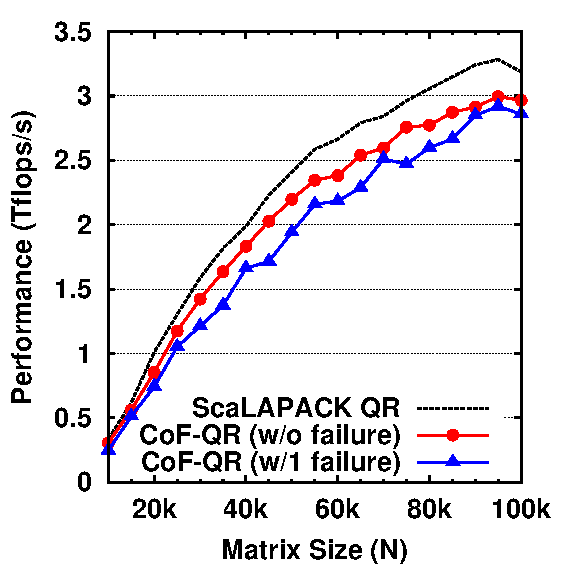
\includegraphics[width=\linewidth]{figures/kraken_new_data}
	\vspace{-.6cm}\caption{ABFT QR and one \cof recovery on Kraken (Lustre).}%($24\times 24$ grid)
	\label{fig:kraken_performance}	
\end{minipage}
\hfill
\begin{minipage}[t]{.29\linewidth}
    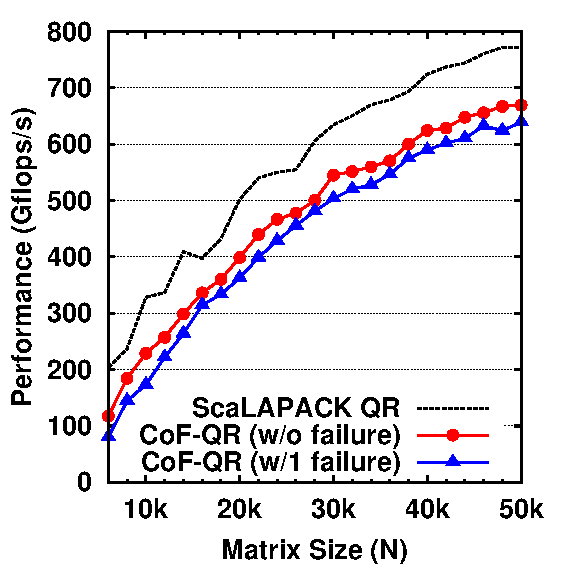
\includegraphics[width=\linewidth]{figures/dancer_performance_data}
	\vspace{-.6cm}\caption{ABFT QR and one \cof recovery on Dancer (local SSD).} %($16\times 8$ grid)
    \label{fig:dancer_performance}
\end{minipage}
\hfill
\begin{minipage}[t]{.29\linewidth}
    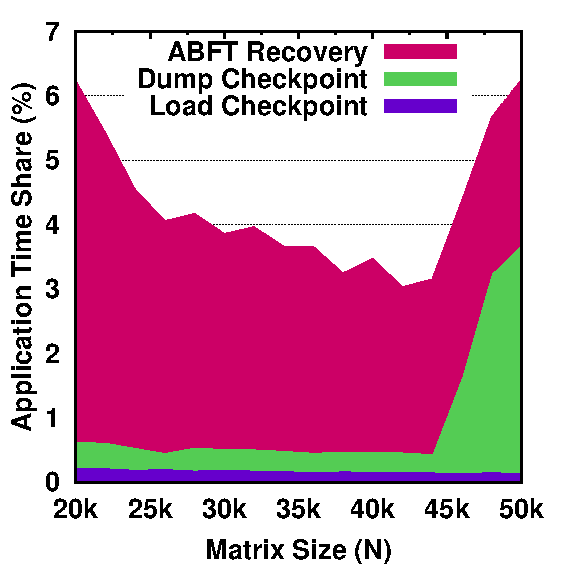
\includegraphics[width=\linewidth]{figures/dancer_1_error_timing_process_new_data}
	\vspace{-.6cm}\caption{Time breakdown of one \cof recovery on Dancer (local SSD).}
    \label{fig:dancer_timing}
\end{minipage}\vspace{-.3cm}
\end{figure}

\subsection{Checkpoint-on-Failure QR Performance}

\paragraph*{Supercomputer Performance:}
Figure~\ref{fig:kraken_performance} presents the performance on the
Kraken supercomputer. The process grid is $24\times 24$ and the block size
is 100. The \cof-QR (no failure) presents the performance of the \cof QR
implementation, in a fault-free execution; it is noteworthy, that when
there are no failures, the performance is exactly identical to the
performance of the unmodified FT-QR implementation. The \cof-QR (with
failure) curves present the performance when a failure is injected after
the first step of the PDLARFB kernel. The performance of the non-fault
tolerant ScaLAPACK QR is also presented for reference.

Without failures, the performance overhead compared to the regular
ScaLAPACK is caused by the extra computation to maintain the checksums inherent to the \abft
algorithm~\cite{pengduppopp12}; this extra computation is unchanged between \cof-QR and
FT-QR. Only on runs where a failure happened do the \cof protocols
undergoe the supplementary overhead of storing and reloading
checkpoints. However, the performance of the \cof-QR remains very
close to the no-failure case. For instance, at matrix size N=100,000,
\cof-QR still achieves 2.86 Tflop/s after recovering from a failure,
which is 90\% of the performance of the non-fault tolerant ScaLAPACK QR.
This demonstrates that the \cof protocol enables efficient, practical
recovery schemes on supercomputers.

\paragraph*{Impact of Local Checkpoint Storage:}

Figure~\ref{fig:dancer_performance} presents the performance of the \cof-QR 
implementation on the Dancer cluster with a $8\times 16$ process
grid. Although a smaller test platform, the Dancer cluster features
local storage on nodes and a variety of performance analysis tools
unavailable on Kraken. As expected (see~\cite{pengduppopp12}), the \abft
method has a higher relative cost on this smaller machine. Compared to
the Kraken platform, the relative cost of \cof failure recovery is
smaller on Dancer. The \cof protocol incurs disk accesses to store and
load checkpoints when a failure hits, hence the recovery overhead
depends on I/O performance. By breaking down the relative cost of each
recovery step in \cof, Figure~\ref{fig:dancer_timing} shows that
checkpoint saving and loading only take a small percentage of the total
run-time, thanks to the availability of solid state disks on every node.
Since checkpoint reloading immediately follows checkpointing, the OS
cache satisfy most disk access, resulting in high I/O performance. For
matrices larger than N=44,000, the memory usage on each node is high and
decrease the available space for disk cache, explaining the decline in
I/O performance and the higher cost of checkpoint management. Overall,
the presence of fast local storage can be leveraged by the \cof protocol
to speedup recovery (unlike periodic checkpointing, which
depends on remote storage by construction). Nonetheless, as demonstrated by the
efficiency on Kraken, while this is a valuable optimization, it is not a
mandatory requirement for satisfactory performance.

%On a problem of this size, the additional overheads
%are dominated by the time it takes to terminate the failing MPI
%application and relaunch a new one. 

%\section{Related Work}
\label{sect:related}

Efforts toward fault tolerance in MPI have previously been attempted.  Automatic
fault tolerance~\cite{Bouteiller10Redesign,MPICHVblocking} is a compelling
approach for users, as failures are completely masked and handled internally by
the MPI library, which requires no new interfaces to MPI or application code
changes. Unfortunately, many recent studies point out that automatic approaches,
either based on checkpoints or replication, will exhibit poor efficiency on
Exaflop platforms~\cite{BOSILCA-2012-696154,lawn265}.

Application Based Fault Tolerance
(ABFT)~\cite{fthpl2011,pengduppopp12,huang1984algorithm} is another approach
that promises better scalability, at the cost of significant algorithm and 
application code changes. Despite some limited 
successes~\cite{europar12/onfailureckpt,Gropp:2004:FTM:1080704.1080714},
MPI interfaces need to be extended to effectively support ABFT. The most notable past 
effort is FT-MPI~\cite{fagg2000ft}, which provided several recovery modes for the user 
but was never standardized and therefore was not portable enough for most users.
\section{Conclusion}
\label{sect:conclusion}

Many responsible voices agree that sharp increases in the volatility of future,
extreme scale computing platforms are likely to imperil our ability to use them
for advanced applications that deliver meaningful scientific results and
maximize research productivity. Since MPI is currently, and will likely continue
to be -- in the medium-term -- both the de-facto programming model for
distributed applications and the default execution model for large scale
platforms running at the bleeding edge, it is the place in the software
infrastructure where semantic and run-time support for application faults needs
to be provided.

The \ulfm proposal is a careful but important step forward toward accomplishing
this goal delivering support for a number of new and innovative resilience
techniques through simple, familiar API calls, but it is backward compatible
with previous versions of the MPI standard, so that non fault-tolerant
applications (legacy or otherwise) are supported without any changes to the
code. Perhaps most significantly, applications can use \ulfm-enabled MPI without
experiencing any degradation in their performance, as we demonstrate in this
paper. Some of these applications along with other portable libraries are
currently being refactored to take advantage of \ulfm semantics.

The author would like to acknowledge his co-authors in the full
paper~\cite{Bland:2012tp}: Aurelien Bouteiller, Thomas Herault, Joshua Hursey,
George Bosilca, and Jack J. Dongarra.

\pagebreak

\newcommand{\BIBdecl}{\setlength{\itemsep}{0.03\baselineskip}} 
\bibliographystyle{IEEEtran}
%\bibliographystyle{plain}
\bibliography{ft-ondemand}

\end{document}

